
\documentclass{article}
\usepackage{graphicx}
\usepackage{tikz}


\begin{document}


%%%%%%%%%%%%%%%%%%%%%%%%%%%%%%%%%%%%%%%%%%%%%%%%%%%%%%%%%
\definecolor{bgcolor}{rgb}{0.98, 0.98, 1.0}
\newenvironment{tikzbox}
{\begin{tikzpicture}
    \node[fill=bgcolor,rounded corners=1em,draw=black,minimum width=0.9\linewidth]}
  {;\end{tikzpicture}}

%%%%%%%%%%%%%%%%%%%%%%%%%%%%%%%%%%%%%%%%%%%%%%%%%%%%%%%%%


\begin{figure}[ht!]
  %\vspace{-1.0em}
\begin{center}
  \begin{tikzbox} {
  \begin{tikzpicture}[minimum width=0]
    \tikzstyle{label} = [node distance = 1.4cm,text=blue]
    \tikzstyle{mycoord} = [node distance = 0cm]
    \tikzstyle{block} = [node distance = 0.5cm,rounded corners=.00cm,
    inner sep=.1cm, fill=bgcolor, minimum height=2em,minimum width=7em]
     \node[block,name=ns1] {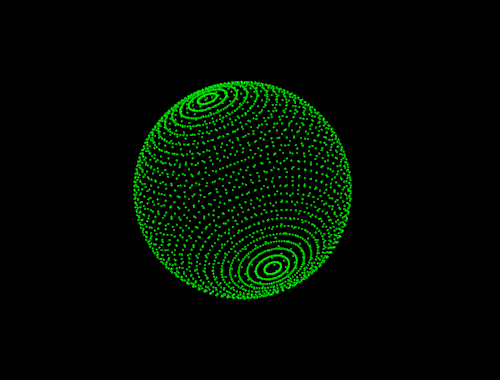
\includegraphics[width=0.25\textwidth]{./sampling_naive_sphere.png} };
     \node[block,xshift=3.5cm,name=ns2] {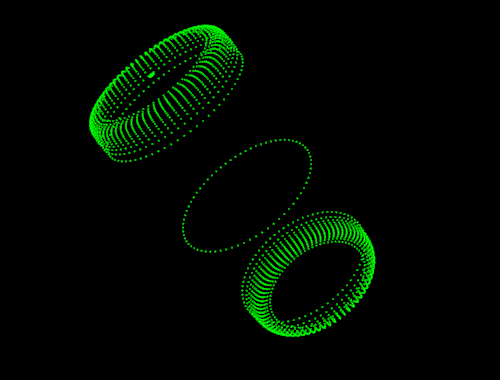
\includegraphics[width=0.25\textwidth]{./sampling_naive_cylinder.png} };
     \node[block,xshift=7cm,name=ns3] {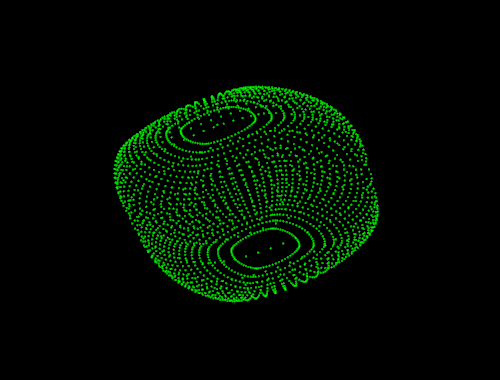
\includegraphics[width=0.25\textwidth]{./sampling_naive_superellipsoid.png} };
     \node[block,xshift=10.5cm,name=ns4] {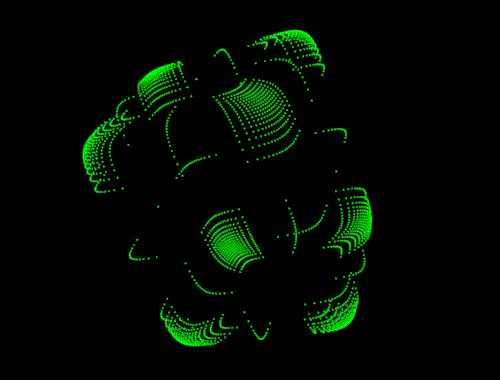
\includegraphics[width=0.25\textwidth]{./sampling_naive_box.png} };

     \node[label,above of=ns1]{Sphere};  
     \node[label,above of=ns2]{Cylinder};
     \node[label,above of=ns3]{Oval shape};
     \node[label,above of=ns4]{Box};


     \node[label,below of=ns1]{$\epsilon_{1} = 1.0, \epsilon_{2}=1.0$};  
     \node[label,below of=ns2]{$\epsilon_{1} = 0.1, \epsilon_{2}=1.0$};
     \node[label,below of=ns3]{$\epsilon_{1} = 0.75, \epsilon_{2}=0.75$};
     \node[label,below of=ns4]{$\epsilon_{1} = 0.1, \epsilon_{2}=0.1$};


  \end{tikzpicture}
  }\end{tikzbox}
\caption{Naive sampling}
\label{fig:coverImage}
\end{center}
\vspace{-2.0em}
\end{figure}



\begin{figure}[ht!]
  %\vspace{-1.0em}
\begin{center}
  \begin{tikzbox} {
  \begin{tikzpicture}[minimum width=0]
    \tikzstyle{label} = [node distance = 1.4cm,text=blue]
    \tikzstyle{mycoord} = [node distance = 0cm]
    \tikzstyle{block} = [node distance = 0.5cm,rounded corners=.00cm,
    inner sep=.1cm, fill=bgcolor, minimum height=2em,minimum width=7em]
     \node[block,name=us1] {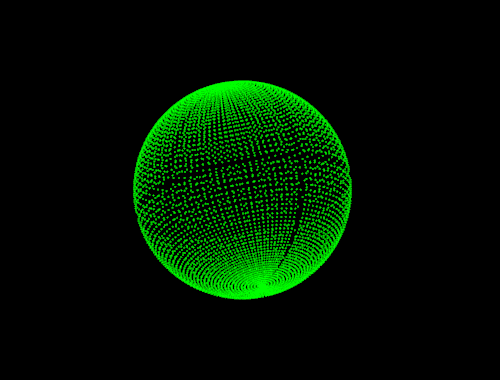
\includegraphics[width=0.25\textwidth]{./sampling_uniform_sphere.png} };
     \node[block,xshift=3.5cm,name=us2] {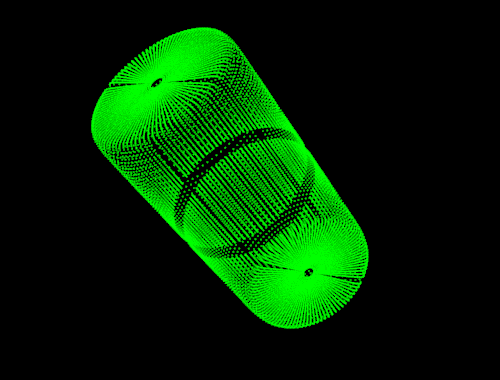
\includegraphics[width=0.25\textwidth]{./sampling_uniform_cylinder.png} };
     \node[block,xshift=7cm,name=us3] {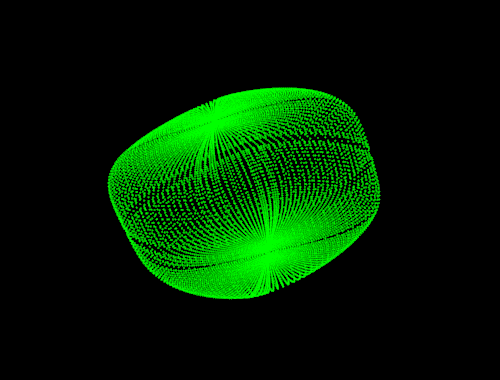
\includegraphics[width=0.25\textwidth]{./sampling_uniform_superellipsoid.png} };
     \node[block,xshift=10.5cm,name=us4] {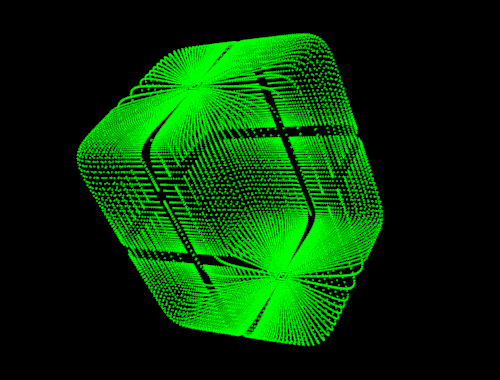
\includegraphics[width=0.25\textwidth]{./sampling_uniform_box.png} };

     \node[label,above of=us1]{Sphere};  
     \node[label,above of=us2]{Cylinder};
     \node[label,above of=us3]{Oval shape};
     \node[label,above of=us4]{Box};


     \node[label,below of=ns1]{$\epsilon_{1} = 1.0, \epsilon_{2}=1.0$};  
     \node[label,below of=ns2]{$\epsilon_{1} = 0.1, \epsilon_{2}=1.0$};
     \node[label,below of=ns3]{$\epsilon_{1} = 0.75, \epsilon_{2}=0.75$};
     \node[label,below of=ns4]{$\epsilon_{1} = 0.1, \epsilon_{2}=0.1$};


  \end{tikzpicture}
  }\end{tikzbox}
\caption{Uniform sampling}
\label{fig:coverImage}
\end{center}
\vspace{-2.0em}
\end{figure}




\end{document}